% ============================================================
% Section 5.4: System Integration and Mode Switching Performance
% ============================================================
\section{System Integration and Mode Switching Performance}
\label{sec:system_integration_mode_switching}

The core innovation of this project lies in integrating two separate assistive functions---mobility and communication---into a single unified medical platform using a single EOG acquisition circuit and a central processing algorithm. To evaluate this integration, the performance of the mode-switching logic between Wheelchair Mode and Virtual Keyboard Mode was tested.

To prevent accidental switching between modes, the system was designed to respond to a specific voluntary blink sequence as a safety toggle switch. Experimental testing confirmed that the MATLAB processing algorithm detected this sequence accurately, switching states immediately without lag or command overlap.

Figure \ref{fig:wheelchair_mode_user_interface} shows the user interface when Wheelchair Mode is activated. As displayed in the interface, the system enters a ``STANDBY'' state upon switching. This software safety feature prevents sudden wheelchair movement until an explicit confirmation command is received, protecting the user when transitioning between communication and navigation modes.

\begin{figure}[H]
  \centering
  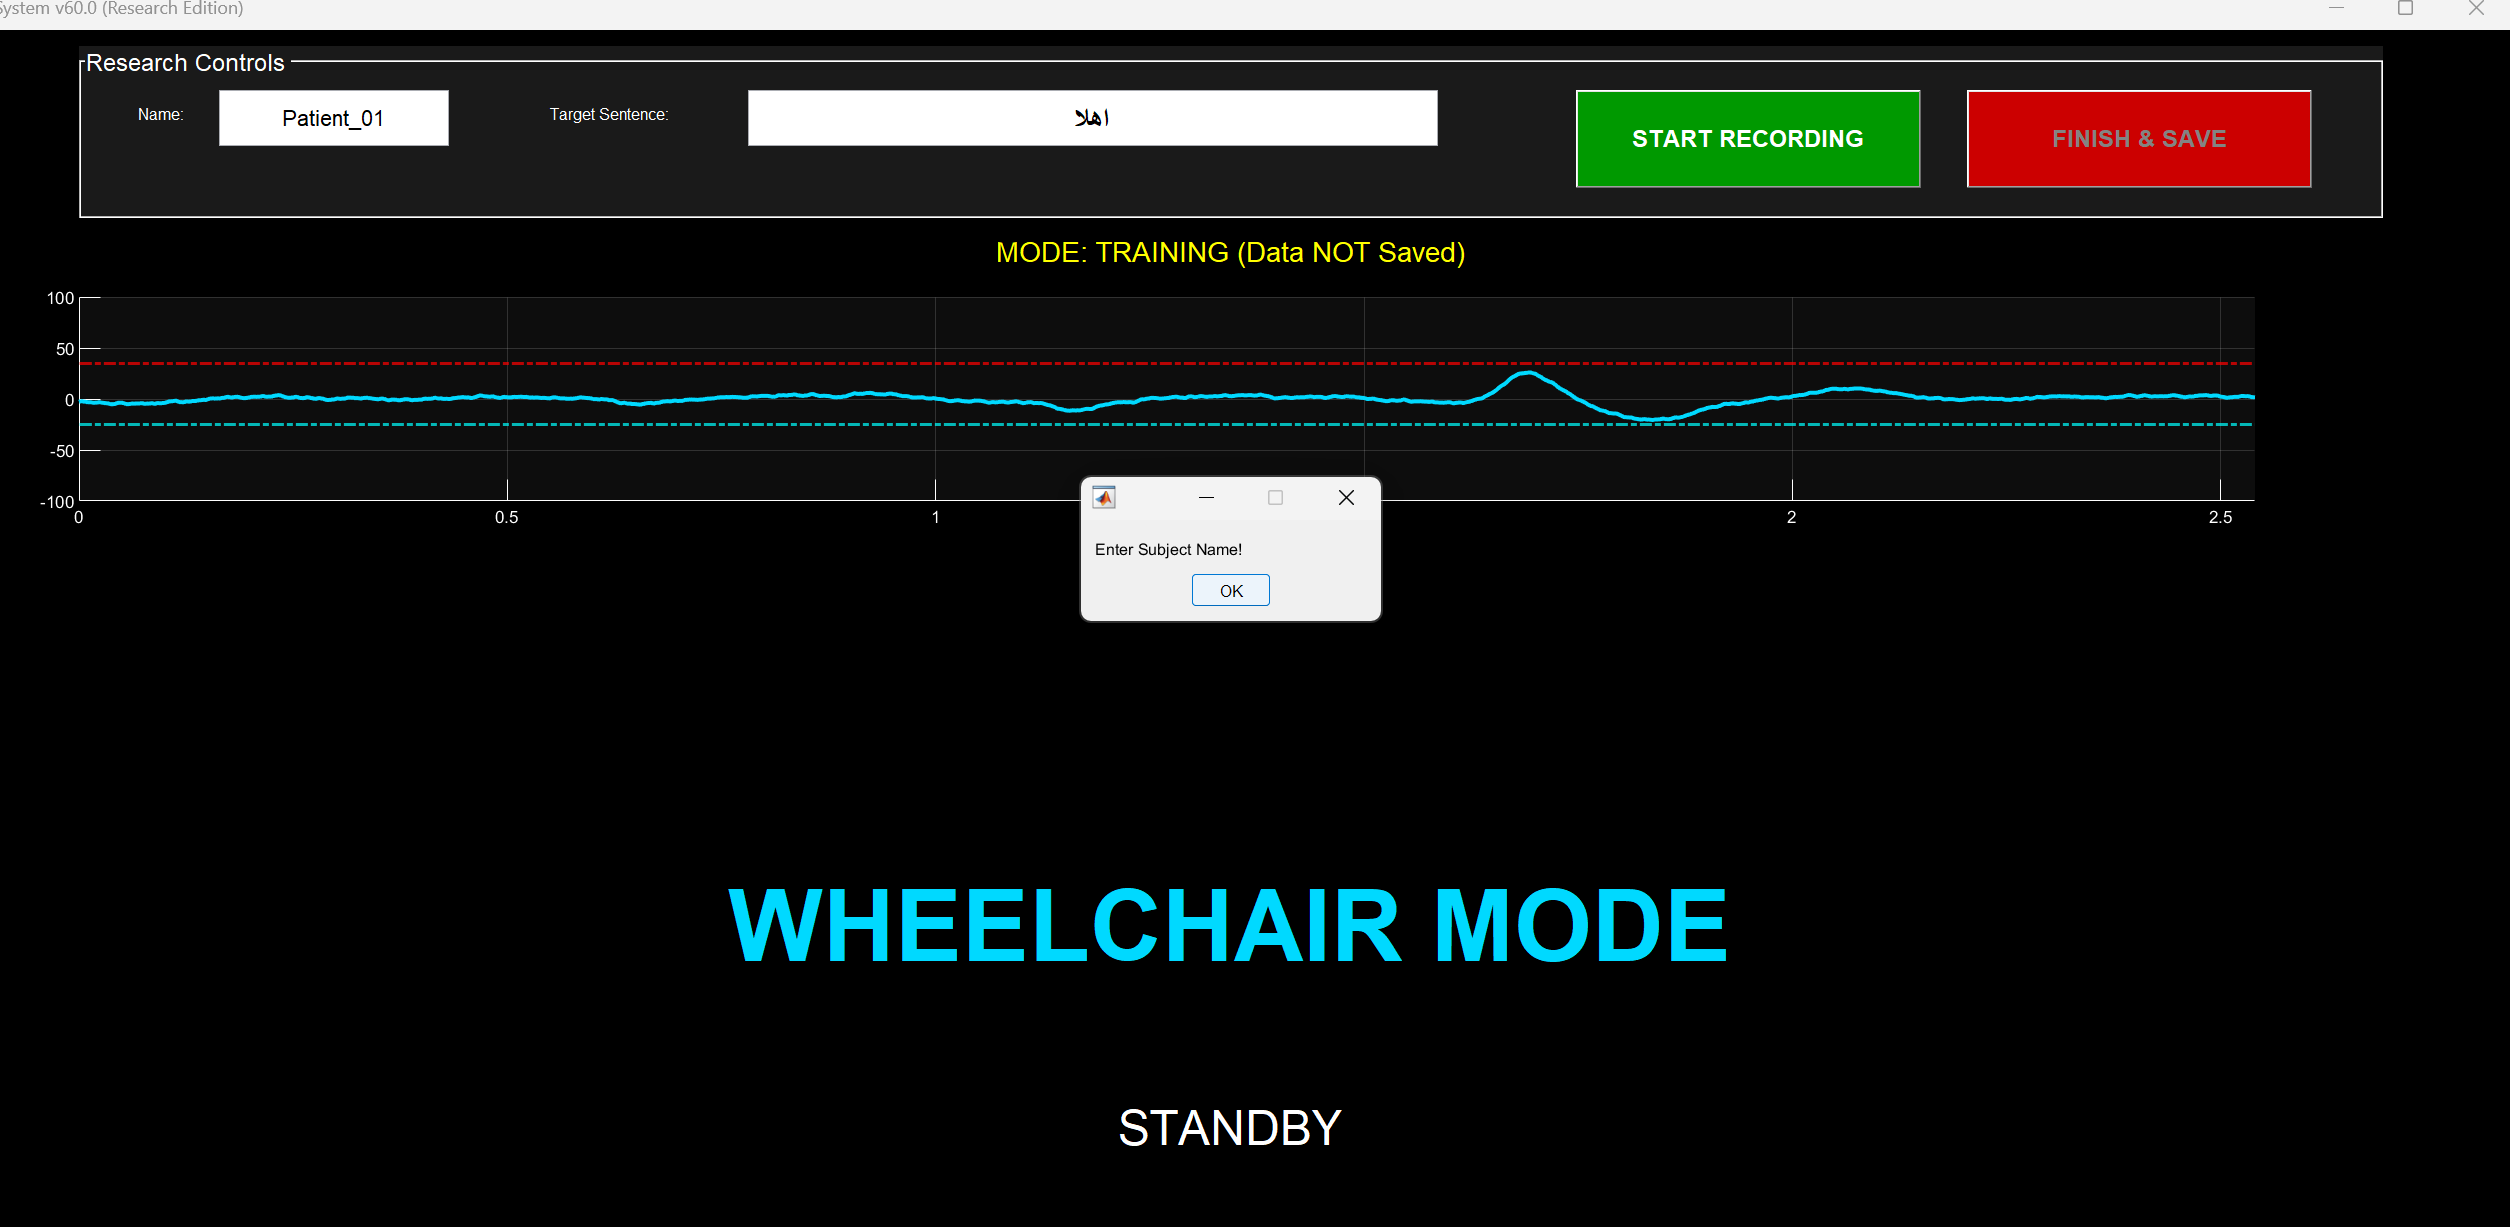
\includegraphics[width=0.85\textwidth]{03_Figures/Ch5/wheelchair_mode_user_interface.png}
  \caption{User interface in Wheelchair Mode.}
  \label{fig:wheelchair_mode_user_interface}
\end{figure}

This integration demonstrated the success of the hybrid system architecture. The user was able to navigate using simple consecutive short blinks (1, 2, or 3 blinks to trigger context-aware directional states), switch smoothly to the virtual keyboard to type using 4 consecutive blinks, and return to navigation using the same EOG interface. This unified design reduces overall hardware costs and minimizes the user's cognitive load by using a single, consistent interface.
